 
%%
%% This is file `sample-sigchi.tex',
%% generated with the docstrip utility.
%%
%% The original source files were:
%%
%% samples.dtx  (with options: `sigchi')
%% 
%% IMPORTANT NOTICE:
%% 
%% For the copyright see the source file.
%% 
%% Any modified versions of this file must be renamed
%% with new filenames distinct from sample-sigchi.tex.
%% 
%% For distribution of the original source see the terms
%% for copying and modification in the file samples.dtx.
%% 
%% This generated file may be distributed as long as the
%% original source files, as listed above, are part of the
%% same distribution. (The sources need not necessarily be
%% in the same archive or directory.)
%%
%% The first command in your LaTeX source must be the \documentclass command.
\documentclass[sigchi]{acmart}

\usepackage{spverbatim}
\usepackage{graphicx}

%%
%% \BibTeX command to typeset BibTeX logo in the docs
\AtBeginDocument{%
	\providecommand\BibTeX{{%
			\normalfont B\kern-0.5em{\scshape i\kern-0.25em b}\kern-0.8em\TeX}}}

%% Rights management information.  This information is sent to you
%% when you complete the rights form.  These commands have SAMPLE
%% values in them; it is your responsibility as an author to replace
%% the commands and values with those provided to you when you
%% complete the rights form.
\setcopyright{acmcopyright}
\copyrightyear{2018}
\acmYear{2018}
\acmDOI{10.1145/1122445.1122456}

%% These commands are for a PROCEEDINGS abstract or paper.
%\acmConference[Woodstock '18]{Woodstock '18: ACM Symposium on Neural%
%	Gaze Detection}{June 03--05, 2018}{Woodstock, NY}
%\acmBooktitle{Woodstock '18: ACM Symposium on Neural Gaze Detection,
%	June 03--05, 2018, Woodstock, NY}
%\acmPrice{15.00}
%\acmISBN{978-1-4503-9999-9/18/06}


%%
%% Submission ID.
%% Use this when submitting an article to a sponsored event. You'll
%% receive a unique submission ID from the organizers
%% of the event, and this ID should be used as the parameter to this command.
%%\acmSubmissionID{123-A56-BU3}

%%
%% The majority of ACM publications use numbered citations and
%% references.  The command \citestyle{authoryear} switches to the
%% "author year" style.
%%
%% If you are preparing content for an event
%% sponsored by ACM SIGGRAPH, you must use the "author year" style of
%% citations and references.
%% Uncommenting
%% the next command will enable that style.
%%\citestyle{acmauthoryear}

%%
%% end of the preamble, start of the body of the document source.
\begin{document}
	
	%%
	%% The "title" command has an optional parameter,
	%% allowing the author to define a "short title" to be used in page headers.
	\title{Natural Language Processing CZ4045}
	\subtitle{Group Report (G20C)}
	
	%%
	%% The "author" command and its associated commands are used to define
	%% the authors and their affiliations.
	%% Of note is the shared affiliation of the first two authors, and the
	%% "authornote" and "authornotemark" commands
	%% used to denote shared contribution to the research.
	\author{Ben Trovato}
	\authornote{Both authors contributed equally to this research.}
	\email{trovato@corporation.com}
	\orcid{1234-5678-9012}
	\author{G.K.M. Tobin}
	\authornotemark[1]
	\email{webmaster@marysville-ohio.com}
	\affiliation{%
		\institution{Institute for Clarity in Documentation}
		\streetaddress{P.O. Box 1212}
		\city{Dublin}
		\state{Ohio}
		\postcode{43017-6221}
	}
	
	\author{Lars Th{\o}rv{\"a}ld}
	\affiliation{%
		\institution{The Th{\o}rv{\"a}ld Group}
		\streetaddress{1 Th{\o}rv{\"a}ld Circle}
		\city{Hekla}
		\country{Iceland}}
	\email{larst@affiliation.org}
	
	\author{Valerie B\'eranger}
	\affiliation{%
		\institution{Inria Paris-Rocquencourt}
		\city{Rocquencourt}
		\country{France}
	}
	
	\author{Aparna Patel}
	\affiliation{%
		\institution{Rajiv Gandhi University}
		\streetaddress{Rono-Hills}
		\city{Doimukh}
		\state{Arunachal Pradesh}
		\country{India}}
	
	\author{Huifen Chan}
	\affiliation{%
		\institution{Tsinghua University}
		\streetaddress{30 Shuangqing Rd}
		\city{Haidian Qu}
		\state{Beijing Shi}
		\country{China}}
	
	\author{Charles Palmer}
	\affiliation{%
		\institution{Palmer Research Laboratories}
		\streetaddress{8600 Datapoint Drive}
		\city{San Antonio}
		\state{Texas}
		\postcode{78229}}
	\email{cpalmer@prl.com}
	
	\author{John Smith}
	\affiliation{\institution{The Th{\o}rv{\"a}ld Group}}
	\email{jsmith@affiliation.org}
	
	\author{Julius P. Kumquat}
	\affiliation{\institution{The Kumquat Consortium}}
	\email{jpkumquat@consortium.net}
	
	%%
	%% By default, the full list of authors will be used in the page
	%% headers. Often, this list is too long, and will overlap
	%% other information printed in the page headers. This command allows
	%% the author to define a more concise list
	%% of authors' names for this purpose.
	% \renewcommand{\shortauthors}{Trovato and Tobin, et al.}
	
	%%
	%% The abstract is a short summary of the work to be presented in the
	%% article.
	\begin{abstract}
		Our task covered data processing on a dataset provided by the review platform \textit{yelp}. We had to analyze the data
		descriptively and we had to focus on the Adjectives in the reports. Therefore we had to compare different methods on how the reviews can be represented by adjectives, which also became our application model. In our application model we were able to find specific properties of the business reviewed in the data.
	\end{abstract}
	
	%%
	%% The code below is generated by the tool at http://dl.acm.org/ccs.cfm.
	%% Please copy and paste the code instead of the example below.
	%%
	\begin{CCSXML}
		<ccs2012>
		<concept>
		<concept_id>10010520.10010553.10010562</concept_id>
		<concept_desc>Computer systems organization~Embedded systems</concept_desc>
		<concept_significance>500</concept_significance>
		</concept>
		</ccs2012>
	\end{CCSXML}
	
	\ccsdesc[500]{Natural Language Processing~Group Assignment}

	
	%%
	%% Keywords. The author(s) should pick words that accurately describe
	%% the work being presented. Separate the keywords with commas.
	\keywords{datasets, neural networks, gaze detection, text tagging}
	
	
	%%
	%% This command processes the author and affiliation and title
	%% information and builds the first part of the formatted document.
	\maketitle
	
	\section{Dataset Analysis}
	\subsection{Writing Style}
	For the sentence segmentation we used the library spacy. Each category is displayed in the graph below.
	\begin{center}
		\begin{table}[!h]
			\caption{Average length of the sentences in the different star categories}
			\begin{tabular}{ c c c c c}
				1 Star & 2 Star & 3 Star  & 4 Star & 5 Star\\
				30.5 & 25.9 & 24.0  & 25 & 24\\
			\end{tabular}
		\end{table}
	\end{center}
	
	\begin{figure}
		\caption{Histograms of the length of the sentences}
		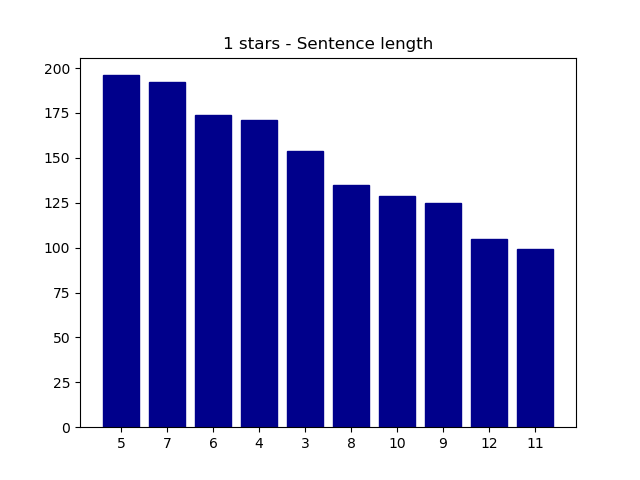
\includegraphics[scale=0.3]{figures/1stars-Sentencelength.png}
		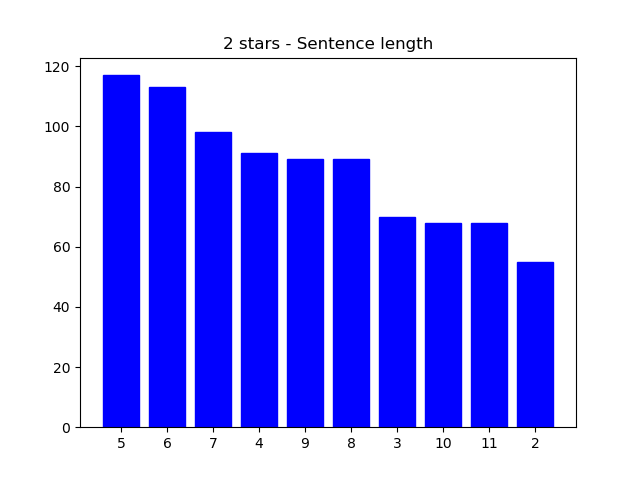
\includegraphics[scale=0.3]{figures/2stars-Sentencelength.png}
		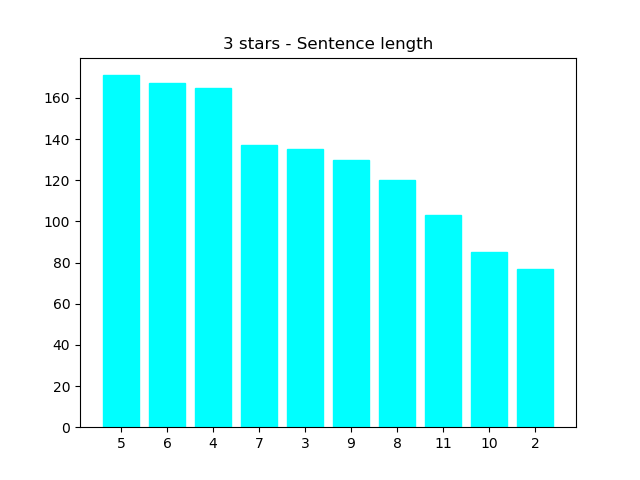
\includegraphics[scale=0.3]{figures/3stars-Sentencelength.png}
		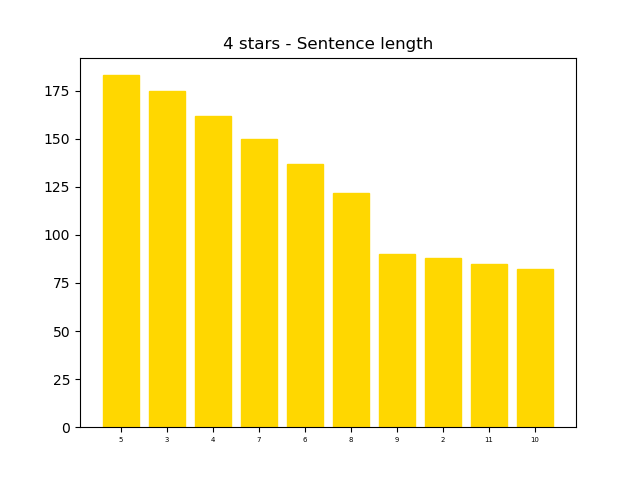
\includegraphics[scale=0.3]{figures/4stars-Sentencelength.png}
		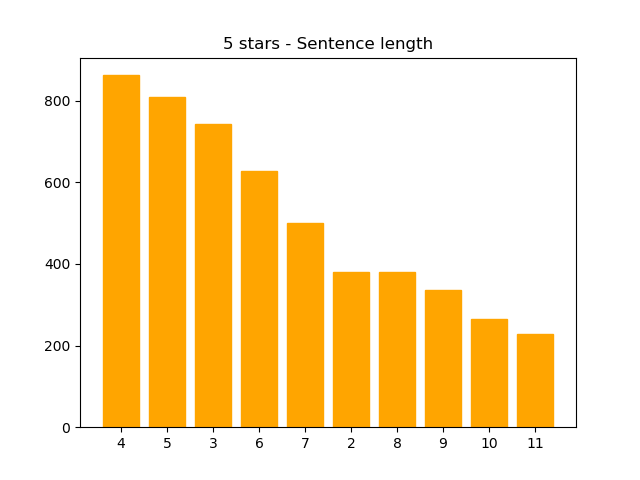
\includegraphics[scale=0.3]{figures/5stars-Sentencelength.png}
	\end{figure}
	As can be seen, the length of sentences is on average longer with a poor rating than with a good rating. 
	
	\subsection{Sentence Segmentation}
	\subsection{Tokenization and Stemming}
	\subsection{POS Tagging}
	\subsection{Most Frequent Adjectives for each Rating}
	\section{Development of a〈Noun - Adjective〉Pair Summarizer}
	For the extraction of the Noun-Adjectives, we used a dependency-grammar approach. In dependency grammar, adjectives are labeled as 'amod'(sources) for sentences like "... bad service ..." while in the case of Adjectives in sentences like "... the service at ... is bad ...", the adjectives are labeled as 'acomp'. With this labels we were able to identify the adjectives. For the nouns we searched the dependency tree of the parent node of the adjective for 
	the 'nsubj' relation. All of these relations were being stored in an array. After another check of the POS-Tag of the collected 'nsubj' relations, we were able to write the ADJ-NOUN Tuples to the final array. Before the adding we lemmatized the words so we can have more accurate number of the used words in the final. We decided to do so since our corpus is to small to distinct between different tenses and therefore increasing the accuracy for the summary of the used adjectives and nouns. The lemmatization was done after the Adjective and Noun were identified For the research we looked at the top twenty appearing pairs.
	In the results we were able to see some characteritics of the reviewed business. It  was possible for example, to make an assumption about the business of the following review:
	'''
	Results oLb3-eXUFtCFJl2DuBhcvA
	[(('front', 'desk'), 20), (('free', 'wifi'), 5), (('clean', 'room'), 5), (('next', 'day'), 5), (('next', 'door'), 4), (('light', 'sleeper'), 4), (('rental', 'car'), 3), (('friendly', 'staff'), 3), (('comfortable', 'bed'), 3), (('great', 'breakfast'), 3), (('hot', 'food'), 3), (('free', 'breakfast'), 3), (('continental', 'breakfast'), 3), (('clean', 'rooms'), 3), (('new', 'room'), 3), (('next', 'morning'), 3), (('complimentary', 'breakfast'), 3), (('free', 'shuttle'), 3), (('first', 'night'), 3), (('first', 'day'), 2)]
	'''
	Here we were able to assume, that the review describes an hotel. Some other reviews also indicated the sector of the business. 
	'''
	Results 2xrpo-LXV9uGIwpvy0dwUw
	[(('clean', 'car'), 4), (('other', 'locations'), 3), (('great', 'job'), 3), (('basic', 'wash'), 2), (('terrible', 'wash'), 2), (('poor', 'job'), 2), (('high', 'pressure'), 2), (('terrible', 'job'), 2), (('helpful', 'guy'), 2), (('horrible', 'service'), 2), (('bad', 'service'), 2), (('worth', 'place'), 2), (('different', 'options'), 2), (('only', 'place'), 2), (('friendly', 'staff'), 2), (('terrible', 'service'), 2), (('horrible', 'smell'), 2), (('happy', 'camper'), 2), (('classic', 'wash'), 2), (('synthetic', 'change'), 2)]
	'''
	It was also possible to identify the kind of food which is served in some restaurants, like mexican, vietnamese or chinese for example.
	'''
	Results DcfkRb2bS2c8z21WH-aS6A
	[(('carne', 'asada'), 13), (('mexican', 'food'), 5), (('free', 'chips'), 4), (('great', 'place'), 4), (('authentic', 'food'), 3), (('red', 'sauce'), 3), (('mexican', 'restaurants'), 3), (('good', 'food'), 3), (('friendly', 'staff'), 3), (('best', 'food'), 3), (('little', 'flavor'), 2), (('toasted', 'bread'), 2), (('iced', 'tea'), 2), (('reasonable', 'price'), 2), (('many', 'restaurants'), 2), (('many', 'people'), 2), (('good', 'salsa'), 2), (('great', 'tacos'), 2), (('good', 'taco'), 2), (('favorite', 'place'), 2)]
	'''
	\begin{verbatim}
	Results c1_adyjYG6JEa1PZAXMOBg
	[(('south', 'indian'), 14), (('indian', 'food'), 14), (('indian', 'restaurant'), 5), (('other', 'places'), 4), (('first', 'time'), 4), (('friendly', 'staff'), 4), (('good', 'food'), 4), (('first', 'experience'), 3), (('high', 'price'), 3), (('second', 'time'), 3), (('indian', 'buffet'), 3), (('great', 'taste'), 2), (('crispy', 'dosa'), 2), (('last', 'night'), 2), (('indian', 'place'), 2), (('great', 'place'), 2), (('delicious', 'food'), 2), (('decent', 'reviews'), 2), (('indian', 'cuisine'), 2), (('tasty', 'food'), 2)]
	\end{verbatim}
	
	\begin{spverbatim}
	Results R4EhR8xhONLFqqI6ZnzNWw
	[(('good', 'dumpling'), 8), (('good', 'food'), 8), (('korean', 'food'), 7), (('korean', 'dishes'), 7), (('steamed', 'dumplings'), 6), (('chinese', 'food'), 5), (('chinese', 'dumplings'), 4), (('chinese', 'cuisine'), 4), (('korean', 'soup'), 4), (('great', 'service'), 4), (('fried', 'pork'), 4), (('huge', 'fan'), 3), (('cheap', 'food'), 3), (('awesome', 'dumpling'), 3), (('fresh', 'noodle'), 3), (('north', 'korean'), 3), (('other', 'dishes'), 3), (('fried', 'rice'), 3), (('hidden', 'gem'), 3), (('northern', 'chinese'), 3)]
	\end{spverbatim}
	
	
	
	\begin{center}
		\begin{tabular}{ c c c c c}
			cell1 & cell2 & cell3  & cell2 & cell3\\ 
			cell4 & cell5 & cell6  & cell2 & cell3\\  
			cell7 & cell8 & cell9  & cell2 & cell3   
		\end{tabular}
	\end{center}
	
	
	With this summarizer we were able to find very specific characteristics of the business. There are alot of useful adjectives to specific offers of the restaurant (e.g.: (('best', 'buffet'), 4), (('quick', 'service'), 2), (('good', 'food'), 5)). With this results we can get extract the most important pairs of the reviews. But still there are some pairs which are not useful to extract the main information of the review like time information which are not useful without their contextes (e.g. : ('single', 'time'), 2),(('first', 'night'), 3), (('first', 'day'), 2)). We assume that the reason for this is the ambigousness of 
	the POS-Tagging. Neither NLTK nor spacy where able to distinguish between the function of a determiner and an adjective. Since these time words can also be used in other contextes as adjectives, an exclusion of these words would not be reasonable. There were also some inaccurancies apperearing like  (('tomato', 'sauce'), 3) which are not usefull for the reflection.
	We can conclude, that we can extract alot of useful knowledge from the reviews using this Adjective-Noun-Summarizer. 
	
	\section{Application}
	
\end{document}
\endinput
%%
%% End of file `sample-sigchi.tex'.
 
